% Drawing 80/01-7 -- folder 80, batch 01, archive page 13 (PDF page 14).
% Transcription: au bas de la carte, une construction d'un arrangement de droites : deux horizontales, deux verticales, deux obliques épaisses, deux droites au crayon et deux lignes en tirets ; sur la première horizontale les points $P$, $L$, $B$, $C'$, $N$, sur la seconde $N'$, $C$, $B'$, $L'$, $P'$ ; $A$, $A'$, $Q$, $Q'$, $M$, $M'$, $R$, $R'$ aux autres intersections ; les longueurs $a$, $b$ (en haut) et $a'$, $b'$ (en bas) marquées sur les segments
% Kind: construction of a line arrangement with named points. Method 2 (schematic redraw from the facsimile). Status: ok.
% Notes: Ten lines, every named point computed as the intersection of its lines and every line drawn through those points. Two horizontals (P, L, B, C', N on the first; N', C, B', L', P' on the second), two verticals (through B, A', N', R' and through R, N, A, B', M), the heavy oblique through M', C', A, L', the heavy steep line through Q, L, A', C, M, the pencil line R, C', C, R' (concurrent with the first horizontal and the heavy oblique at C'), the pencil line P, A', A towards P' (dashed on the left of A' as on the page), the dashed line B B', and the dashed arc from Q through Q' to B. P' lies off the right edge, at the meeting of the second horizontal and the line A' A; the label is set where he wrote it. Left out: an overwritten letter at the crossing of the two heavy obliques, above M'. Still differs: on the page the line A' A is interrupted between A and the right half; L and B are 0.3 mm apart, as on the page. Redrawn 2026-11-12 (issue 128): to check again. 2026-11-14, Claude Opus 5.5, overlay check (issue 147): rasterised from its own coordinates over the 400 dpi colour scan on a unit grid and measured (every line within 0.6 unit of its ink on average; all ink of the construction within 1.5 units of a line or label, the calculations at the right excepted); not compiled (no TeX in the session). No change needed: the ten lines, the dashed lines and arc, the points and their labels lie on the page where they are drawn. The interruption of A' A between A and the right half is a property of the page, noted above, not a difference of the redraw. Status set to ok.
% Coordinates: 1 unit = 1 mm = 1/100 of the crop width (bbox in page fractions: [0.2, 0.215, 0.99, 0.52]).
% Redrawn by Claude (claude-fable-5-2), issue #128, 2026-11-12; not checked by a human; not compiled (no TeX in the session).
% Checked by Claude (claude-opus-5-5) 2026-11-14 (issue #147): overlaid on the 400 dpi colour facsimile, corrected; not compiled (no TeX in the session). Not checked by a human. Status: ok.
% Rights: reproduces part of the work -- behind RENDER_TRANSCRIPTS, never published by itself.
\documentclass[tikz,border=3pt]{standalone}
\usepackage{amsmath,amssymb}
\usetikzlibrary{patterns,arrows.meta}
\tikzset{pencil/.style={black!45}, struck/.style={black!35}, mpt/.style={circle,draw,inner sep=1.3pt}, pt/.style={circle,fill,inner sep=0.9pt}, opt/.style={circle,draw,fill=white,inner sep=1.1pt}}
\begin{document}
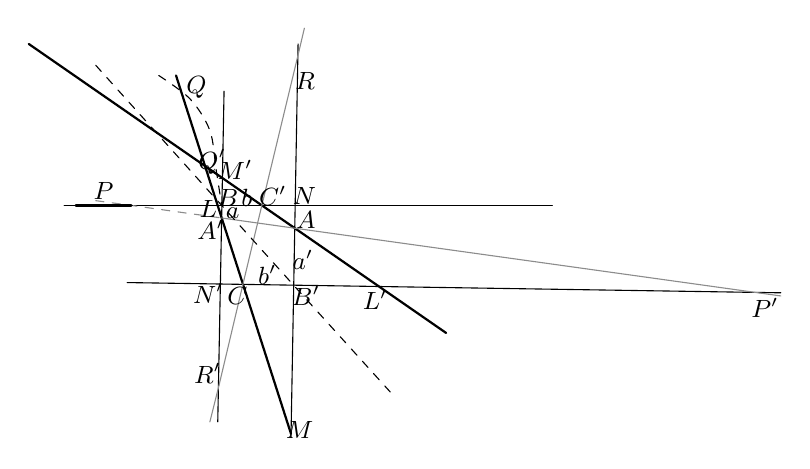
\begin{tikzpicture}[x=1mm,y=1mm,line cap=round,line join=round,font=\scriptsize]
\draw (9,-23.5) -- (71,-23.5);
\draw (17,-33.3) -- (100,-34.6);
\draw (29.3,-9) -- (28.5,-51);
\draw (38.7,-3) -- (37.8,-53);
\draw[thick] (4.5,-3) -- (57.5,-39.7);
\draw[thick] (23.2,-7) -- (29,-25.1) -- (31.7,-33.5) -- (37.8,-52.5);
\draw[pencil] (39.5,-1) -- (38.7,-4.4) -- (34.1,-23.5) -- (31.7,-33.5) -- (28.6,-46.6) -- (27.5,-51);
\draw[pencil] (29,-25.1) -- (38.3,-26.4) -- (100,-35);
\draw[pencil,dashed] (13,-22.9) -- (17.5,-23.5) -- (29,-25.1);
\draw[dashed] (13,-5.7) -- (29,-23.5) -- (38.1,-33.6) -- (50.5,-47.3);
\draw[dashed] plot[smooth, tension=0.55] coordinates {(21,-7) (25,-10) (27.5,-14) (28.3,-19) (29,-23.5)};
\draw[very thick] (10.5,-23.5) -- (17.5,-23.5);
\node[inner sep=1pt] at (14,-21.7) {\small $P$};
\node[inner sep=1pt] at (27.3,-23.9) {\small $L$};
\node[inner sep=1pt] at (29.8,-22.6) {\small $B$};
\node[inner sep=1pt] at (35.5,-22.3) {\small $C'$};
\node[inner sep=1pt] at (39.5,-22.3) {\small $N$};
\node[inner sep=1pt] at (27.3,-34.7) {\small $N'$};
\node[inner sep=1pt] at (31,-35) {\small $C$};
\node[inner sep=1pt] at (39.7,-35) {\small $B'$};
\node[inner sep=1pt] at (48.5,-35.5) {\small $L'$};
\node[inner sep=1pt] at (98,-36.5) {\small $P'$};
\node[inner sep=1pt] at (39.7,-25.3) {\small $A$};
\node[inner sep=1pt] at (27.6,-26.6) {\small $A'$};
\node[inner sep=1pt] at (25.8,-8.5) {\small $Q$};
\node[inner sep=1pt] at (27.8,-18) {\small $Q'$};
\node[inner sep=1pt] at (38.9,-52) {\small $M$};
\node[inner sep=1pt] at (30.7,-19) {\small $M'$};
\node[inner sep=1pt] at (39.6,-7.7) {\small $R$};
\node[inner sep=1pt] at (27.2,-44.8) {\small $R'$};
\node[inner sep=1pt] at (30.4,-24.5) {\small $a$};
\node[inner sep=1pt] at (32.2,-22.6) {\small $b$};
\node[inner sep=1pt] at (39.3,-30.4) {\small $a'$};
\node[inner sep=1pt] at (34.8,-32.3) {\small $b'$};
\end{tikzpicture}
\end{document}
